\documentclass[journal, onecolumn]{IEEEtran}

% --- PACKAGES ---
\usepackage{amsmath}
\usepackage{amssymb}
\usepackage{amsfonts}
\usepackage{amsthm}
\usepackage{graphicx}
\usepackage[utf8]{inputenc}
\usepackage[T1]{fontenc}
\usepackage{url}
\usepackage{xcolor}
\usepackage{enumitem}
\usepackage{tcolorbox}
\usepackage{tikz}
\usepackage{float}
\usepackage{booktabs}
\usepackage{multirow}
\usepackage[normalem]{ulem}
\usetikzlibrary{arrows.meta, positioning, shapes.geometric, calc, decorations.pathreplacing}

% --- USER PREFERENCE COLORS ---
\definecolor{Garnet}{HTML}{73000a}
\definecolor{SecondaryBlue}{HTML}{466A9F}
\definecolor{SecondaryGreen}{HTML}{65780B}
\definecolor{FlatRed}{HTML}{CC2E40}
\definecolor{FlatDark}{HTML}{1F414D}
\definecolor{FlatYellow}{HTML}{CED318}
\definecolor{FlatGold}{HTML}{A49137}
\definecolor{LightGray}{HTML}{F0F0F0}
\definecolor{Rose}{HTML}{CC2E40}

% --- FORMATTING ---
\setlength{\parindent}{0pt}
\setlength{\parskip}{1.2em}
\renewcommand{\baselinestretch}{1.2}

% --- CUSTOM COMMANDS ---
\newcommand{\vocab}[1]{\textbf{\textcolor{Garnet}{#1}}}
\newcommand{\mathhighlight}[1]{\textcolor{SecondaryBlue}{#1}}

% --- TCOLORBOX STYLES ---
\tcbset{
    examplebox/.style={
        colback=LightGray,
        colframe=SecondaryBlue,
        fonttitle=\bfseries,
        title=#1,
        sharp corners,
        boxrule=1pt
    },
    memorybox/.style={
        colback=Garnet!10,
        colframe=Garnet,
        fonttitle=\bfseries,
        title=#1,
        sharp corners,
        boxrule=2pt
    }
}

% --- TITLE & AUTHOR ---
\title{\textcolor{Garnet}{\textbf{Monte Carlo Estimation of Action Values}}\\[0.3em]
\large From $V(s)$ to $Q(s,a)$: Exploration and $\varepsilon$-Greedy Policies}
\author{CSCE 775 -- Reinforcement Learning}
\date{\today}

\begin{document}
\maketitle

% ============================================================
\section{Introduction: From $V(s)$ to $Q(s,a)$}
% ============================================================

In the previous guide on Monte Carlo prediction, we learned how to estimate the \vocab{state-value function} $V(s)$, which tells us how good it is to \textit{be in} a particular state. This is useful for evaluating a policy, but it does not directly tell us which \textit{action} to take. Knowing that a room is valuable does not tell us which door to walk through to get the most reward.

To actually \textit{choose} actions, we need the \vocab{action-value function} $Q(s,a)$, which tells us how good it is to take a specific action $a$ in state $s$ and then follow the policy $\pi$ thereafter. If we know $Q(s,a)$ for all actions, choosing the best action is trivial: just pick $\arg\max_a Q(s,a)$.

\subsection{Why $V(s)$ Alone Is Not Enough}

With only $V(s)$, selecting the best action requires knowing the \textit{model} of the environment. Specifically, we would need to compute the following for each action $a$.
\begin{align}
    \arg\max_a \sum_{s', r} p(s', r \mid s, a) \left[ r + \gamma V(s') \right]
\end{align}
This requires the transition probabilities $p(s', r \mid s, a)$, which we often do not have. With $Q(s,a)$, we bypass this entirely: we just pick $\arg\max_a Q(s,a)$ without needing any model. This is what makes $Q$-values essential for \vocab{model-free} control.

\subsection{Defining $Q^\pi(s,a)$}

The action-value function under policy $\pi$ is defined as follows.
\begin{align}
    Q^\pi(s,a) = \mathbb{E}_\pi\left[G_t \mid S_t = s, A_t = a\right]
\end{align}
Let us unpack each piece of notation. $Q^\pi(s,a)$ is the value of taking action $a$ in state $s$ and then following policy $\pi$ for all subsequent decisions. The symbol $\mathbb{E}_\pi[\cdot]$ means ``the expected value (average) if we follow policy $\pi$ after the first action.'' The term $G_t$ is the return (total discounted reward from time $t$ onward). The condition $S_t = s, A_t = a$ means ``given that we are in state $s$ at time $t$ and take action $a$.''

\begin{tcolorbox}[examplebox={$V(s)$ vs $Q(s,a)$: An Analogy}]
Think of $V(s)$ as a review of a restaurant: ``This place is great!'' It tells you the overall quality, but not what to order. $Q(s,a)$ is like a review of each dish: ``The pizza is excellent, but the pasta is mediocre.'' With dish-level reviews, you can directly choose the best item on the menu without needing to know anything about the kitchen (the model).
\end{tcolorbox}

% ============================================================
\section{The Gridworld with Actions}
% ============================================================

We reuse the same $3 \times 3$ gridworld from the prediction guide. The agent occupies states $S_1$ through $S_9$, where $S_9$ is the terminal goal state. Stepping into $S_9$ yields $R = +10$, and every other step yields $R = -1$. The discount factor is $\gamma = 0.9$. The key difference now is that we explicitly label the agent's \vocab{actions}: Up ($\uparrow$), Down ($\downarrow$), Left ($\leftarrow$), and Right ($\rightarrow$).

\begin{figure}[H]
\centering
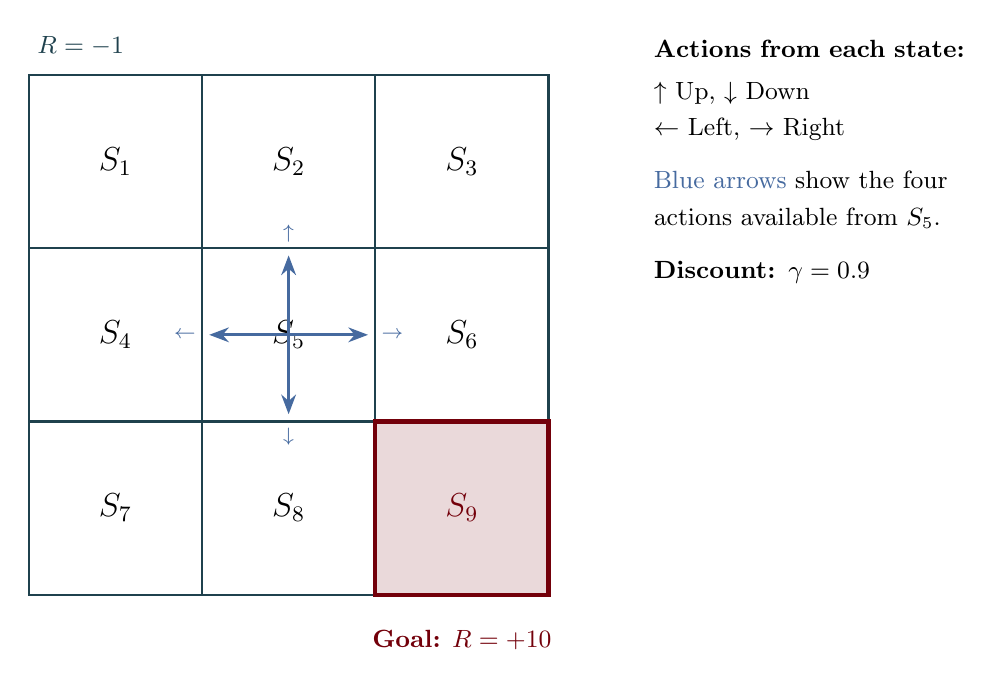
\begin{tikzpicture}[
    cell/.style={minimum size=2.2cm, draw=FlatDark, thick, font=\large},
    goal/.style={cell, fill=Garnet!15, draw=Garnet, line width=1.5pt},
    rlabel/.style={font=\small, FlatDark},
    actarr/.style={-{Stealth[length=2.5mm]}, line width=1pt, SecondaryBlue}
]
% Row 1 (top): S1, S2, S3
\node[cell] (s1) at (0, 4.4) {$S_1$};
\node[cell] (s2) at (2.2, 4.4) {$S_2$};
\node[cell] (s3) at (4.4, 4.4) {$S_3$};
% Row 2: S4, S5, S6
\node[cell] (s4) at (0, 2.2) {$S_4$};
\node[cell] (s5) at (2.2, 2.2) {$S_5$};
\node[cell] (s6) at (4.4, 2.2) {$S_6$};
% Row 3 (bottom): S7, S8, S9
\node[cell] (s7) at (0, 0) {$S_7$};
\node[cell] (s8) at (2.2, 0) {$S_8$};
\node[goal] (s9) at (4.4, 0) {\textcolor{Garnet}{$S_9$}};

% Action arrows from S5 (example state)
\draw[actarr] (s5.center) -- ([yshift=-3pt]s5.north) node[above=1pt, font=\scriptsize, SecondaryBlue] {$\uparrow$};
\draw[actarr] (s5.center) -- ([yshift=3pt]s5.south) node[below=1pt, font=\scriptsize, SecondaryBlue] {$\downarrow$};
\draw[actarr] (s5.center) -- ([xshift=3pt]s5.west) node[left=1pt, font=\scriptsize, SecondaryBlue] {$\leftarrow$};
\draw[actarr] (s5.center) -- ([xshift=-3pt]s5.east) node[right=1pt, font=\scriptsize, SecondaryBlue] {$\rightarrow$};

% Labels
\node[rlabel, above=0.1cm of s1.north west, anchor=south west] {$R = -1$};
\node[rlabel, below=0.3cm of s9] {\textcolor{Garnet}{\textbf{Goal:} $R = +10$}};

% Legend
\node[right=1.2cm of s3, anchor=west, font=\small, text width=4cm] {
    \textbf{Actions from each state:}\\[2pt]
    $\uparrow$ Up, $\downarrow$ Down\\
    $\leftarrow$ Left, $\rightarrow$ Right\\[6pt]
    \textcolor{SecondaryBlue}{Blue arrows} show the four\\
    actions available from $S_5$.\\[6pt]
    \textbf{Discount:} $\gamma = 0.9$
};
\end{tikzpicture}
\caption{The $3\times 3$ gridworld with actions. Each non-terminal state has four actions. Blue arrows illustrate the action set from $S_5$.}
\label{fig:gridworld_actions}
\end{figure}

% ============================================================
\section{A Sample Episode with Actions}
% ============================================================

Consider the same episode from the prediction guide, but now we explicitly record the action taken at each step.

\begin{tcolorbox}[examplebox={Episode Trajectory with Actions}]
$S_1 \xrightarrow{\text{R}} S_2 \xrightarrow{\text{D}} S_5 \xrightarrow{\text{L}} S_4 \xrightarrow{\text{U}}
\textcolor{Rose}{S_1} \xrightarrow{\text{R}} \textcolor{Rose}{S_2} \xrightarrow{\text{R}} S_3 \xrightarrow{\text{D}} S_6 \xrightarrow{\text{D}} S_9$

\medskip
R = Right, D = Down, L = Left, U = Up.\\
States in \textcolor{Rose}{\textbf{rose}} are revisits. Notice that $(S_1, \text{Right})$ and $(S_2, \text{Right})$ are repeated (state, action) pairs, while $(S_2, \text{Down})$ at $t=1$ is a \textit{different} (state, action) pair from $(S_2, \text{Right})$ at $t=5$.
\end{tcolorbox}

\begin{figure}[H]
\centering
\begin{tikzpicture}[
    cell/.style={minimum size=1.8cm, draw=FlatDark!40, thick, font=\large},
    goal/.style={cell, fill=Garnet!15, draw=Garnet, line width=1.5pt},
    arr/.style={-{Stealth[length=3mm]}, line width=1.2pt, FlatDark},
    revisit/.style={-{Stealth[length=3mm]}, line width=1.2pt, Rose},
    step/.style={font=\scriptsize\bfseries, fill=white, inner sep=1pt},
    rstep/.style={font=\scriptsize\bfseries, fill=white, inner sep=1pt, Rose},
    act/.style={font=\tiny, SecondaryBlue, fill=white, inner sep=1pt},
    ract/.style={font=\tiny, Rose, fill=white, inner sep=1pt}
]
% Grid
\node[cell] (s1) at (0, 3.6) {$S_1$};
\node[cell] (s2) at (1.8, 3.6) {$S_2$};
\node[cell] (s3) at (3.6, 3.6) {$S_3$};
\node[cell] (s4) at (0, 1.8) {$S_4$};
\node[cell] (s5) at (1.8, 1.8) {$S_5$};
\node[cell] (s6) at (3.6, 1.8) {$S_6$};
\node[cell] (s7) at (0, 0) {$S_7$};
\node[cell] (s8) at (1.8, 0) {$S_8$};
\node[goal] (s9) at (3.6, 0) {\textcolor{Garnet}{$S_9$}};

% Step 0: S1 -> S2 (Right)
\draw[arr] ([yshift=4pt]s1.east) -- ([yshift=4pt]s2.west)
    node[step, midway, above=2pt] {0}
    node[act, midway, below=0pt] {R};
% Step 1: S2 -> S5 (Down)
\draw[arr] ([xshift=-4pt]s2.south) -- ([xshift=-4pt]s5.north)
    node[step, midway, left=2pt] {1}
    node[act, midway, right=0pt] {D};
% Step 2: S5 -> S4 (Left)
\draw[arr] ([yshift=-2pt]s5.west) -- ([yshift=-2pt]s4.east)
    node[step, midway, below=2pt] {2}
    node[act, midway, above=0pt] {L};
% Step 3: S4 -> S1 (Up)
\draw[arr] ([xshift=4pt]s4.north) -- ([xshift=4pt]s1.south)
    node[step, midway, right=2pt] {3}
    node[act, midway, left=0pt] {U};
% Step 4: S1 -> S2 (Right, revisit)
\draw[revisit] ([yshift=-4pt]s1.east) -- ([yshift=-4pt]s2.west)
    node[rstep, midway, below=2pt] {4}
    node[ract, midway, above=0pt] {R};
% Step 5: S2 -> S3 (Right, revisit of S2)
\draw[revisit] ([yshift=4pt]s2.east) -- ([yshift=4pt]s3.west)
    node[rstep, midway, above=2pt] {5}
    node[ract, midway, below=0pt] {R};
% Step 6: S3 -> S6 (Down)
\draw[arr] ([xshift=4pt]s3.south) -- ([xshift=4pt]s6.north)
    node[step, midway, right=2pt] {6}
    node[act, midway, left=0pt] {D};
% Step 7: S6 -> S9 (Down)
\draw[arr] ([xshift=4pt]s6.south) -- ([xshift=4pt]s9.north)
    node[step, midway, right=2pt] {7}
    node[act, midway, left=0pt] {D};

% Start marker
\node[above=0.25cm of s1, font=\small\bfseries, FlatDark] {START};
\end{tikzpicture}
\caption{Episode path with action labels. Each arrow shows the time step and the action taken. \textcolor{Rose}{Rose arrows} indicate revisited (state, action) pairs.}
\label{fig:episode_path_actions}
\end{figure}

% ============================================================
\section{Computing Returns for (State, Action) Pairs}
% ============================================================

The return computation is identical to the prediction guide. We compute $G_t$ backward from the terminal state using $G_t = R_{t+1} + \gamma\, G_{t+1}$. The difference is that each return is now associated with a \vocab{(state, action) pair} rather than just a state.

\begin{tcolorbox}[examplebox={Backward Return Computation}]
\begin{align}
G_7 &= R_8 = +10 && \text{$(S_6, \text{D}) \to S_9$} \notag\\[4pt]
G_6 &= R_7 + \gamma G_7 = -1 + 0.9(10) = \mathhighlight{8.0} && \text{$(S_3, \text{D})$} \notag\\[4pt]
G_5 &= R_6 + \gamma G_6 = -1 + 0.9(8.0) = \mathhighlight{6.2} && \text{$(S_2, \text{R})$ -- 2nd visit} \notag\\[4pt]
G_4 &= R_5 + \gamma G_5 = -1 + 0.9(6.2) = \mathhighlight{4.58} && \text{$(S_1, \text{R})$ -- 2nd visit} \notag\\[4pt]
G_3 &= R_4 + \gamma G_4 = -1 + 0.9(4.58) = \mathhighlight{3.122} && \text{$(S_4, \text{U})$} \notag\\[4pt]
G_2 &= R_3 + \gamma G_3 = -1 + 0.9(3.122) = \mathhighlight{1.810} && \text{$(S_5, \text{L})$} \notag\\[4pt]
G_1 &= R_2 + \gamma G_2 = -1 + 0.9(1.810) = \mathhighlight{0.629} && \text{$(S_2, \text{D})$} \notag\\[4pt]
G_0 &= R_1 + \gamma G_1 = -1 + 0.9(0.629) = \mathhighlight{-0.434} && \text{$(S_1, \text{R})$ -- 1st visit} \notag
\end{align}
\end{tcolorbox}

\begin{table}[H]
\centering
\caption{Returns $G_t$ for each (state, action) pair in the episode.}
\label{tab:returns_actions}
\begin{tabular}{ccccc}
\toprule
\textbf{Time $t$} & \textbf{State} & \textbf{Action} & \textbf{Return $G_t$} & \textbf{Visit \#} \\
\midrule
0 & $S_1$ & Right  & $-0.434$ & 1st \\
1 & $S_2$ & Down   & $0.629$  & 1st \\
2 & $S_5$ & Left   & $1.810$  & 1st \\
3 & $S_4$ & Up     & $3.122$  & 1st \\
4 & \textcolor{Rose}{$S_1$} & \textcolor{Rose}{Right}  & \textcolor{Rose}{$4.58$}   & \textcolor{Rose}{2nd} \\
5 & \textcolor{Rose}{$S_2$} & \textcolor{Rose}{Right}  & \textcolor{Rose}{$6.2$}    & \textcolor{Rose}{2nd} \\
6 & $S_3$ & Down   & $8.0$    & 1st \\
7 & $S_6$ & Down   & $10.0$   & 1st \\
\bottomrule
\end{tabular}
\end{table}

Notice the critical distinction: $(S_2, \text{Down})$ at $t=1$ and $(S_2, \text{Right})$ at $t=5$ are \textit{different} (state, action) pairs, even though they share the same state. The pair $(S_1, \text{Right})$ appears twice (at $t=0$ and $t=4$), and $(S_2, \text{Right})$ also appears twice if we count $t=5$ as a revisit. Meanwhile, $(S_2, \text{Down})$ appears only once. This is the key difference from state-value estimation: the same state can appear with different actions, and each (state, action) combination is tracked independently.

% ============================================================
\section{First-Visit MC for Action Values}
% ============================================================

\begin{tcolorbox}[memorybox={Definition: First-Visit MC for $Q(s,a)$}]
For each (state, action) pair $(s,a)$ appearing in an episode, record the return $G_t$ only for the \vocab{first time} that specific pair $(s,a)$ is visited. The action-value estimate is the average of these first-visit returns across all episodes.
\begin{align}
    Q(s,a) \approx \frac{1}{N(s,a)} \sum_{i=1}^{N(s,a)} G_t^{(i)} \quad \text{where each } G_t^{(i)} \text{ is from the first visit to } (s,a) \text{ in episode } i
\end{align}
\end{tcolorbox}

The key distinction from the state-value version is that we track \textit{(state, action) pairs}, not just states. Two visits to the same state with different actions count as visits to different pairs. In our episode, $(S_1, \text{Right})$ is visited at $t=0$ and $t=4$. First-visit MC uses only the return from $t=0$. Meanwhile, $(S_2, \text{Down})$ at $t=1$ and $(S_2, \text{Right})$ at $t=5$ are different pairs entirely, so both are first visits.

After processing this single episode, our $Q$-table looks like the following.

\begin{table}[H]
\centering
\caption{$Q$-table after one episode (first-visit MC). Only observed (state, action) pairs have estimates.}
\label{tab:qtable}
\begin{tabular}{lcccc}
\toprule
\textbf{State} & $Q(s, \text{Up})$ & $Q(s, \text{Down})$ & $Q(s, \text{Left})$ & $Q(s, \text{Right})$ \\
\midrule
$S_1$ & --- & --- & --- & $-0.434$ \\
$S_2$ & --- & $0.629$ & --- & $6.2$ \\
$S_3$ & --- & $8.0$ & --- & --- \\
$S_4$ & $3.122$ & --- & --- & --- \\
$S_5$ & --- & --- & $1.810$ & --- \\
$S_6$ & --- & $10.0$ & --- & --- \\
\bottomrule
\end{tabular}
\end{table}

The dashes (---) represent (state, action) pairs that were never visited. We have \textit{no estimate} for these pairs. This is a serious problem that we will address in Section~VII.

\begin{tcolorbox}[examplebox={First-Visit MC for $Q(s,a)$ Pseudocode}]
\texttt{Initialize:} $Q(s,a) \leftarrow 0$, $\text{Returns}(s,a) \leftarrow$ empty list, for all $s, a$\\[4pt]
\texttt{For each episode:}\\
\quad Generate episode: $S_0, A_0, R_1, S_1, A_1, R_2, \ldots, S_T$\\
\quad $G \leftarrow 0$\\
\quad \texttt{For} $t = T-1, T-2, \ldots, 0$:\\
\quad\quad $G \leftarrow R_{t+1} + \gamma G$\\
\quad\quad \texttt{If} $(S_t, A_t)$ not in $\{(S_0,A_0), (S_1,A_1), \ldots, (S_{t-1},A_{t-1})\}$: \hfill \textcolor{Garnet}{$\triangleleft$ first visit only}\\
\quad\quad\quad Append $G$ to $\text{Returns}(S_t, A_t)$\\
\quad\quad\quad $Q(S_t, A_t) \leftarrow \text{average}(\text{Returns}(S_t, A_t))$
\end{tcolorbox}

% ============================================================
\section{Q-Table Visualization}
% ============================================================

The following diagram shows the $Q$-table as a grid where each cell is subdivided into four quadrants, one for each action. This visualization makes it easy to see which (state, action) pairs have been estimated and which remain unknown.

\begin{figure}[H]
\centering
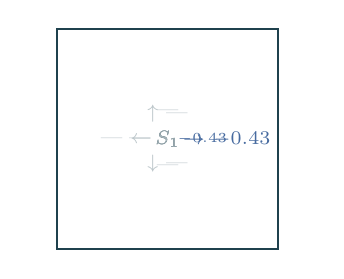
\begin{tikzpicture}[
    cell/.style={minimum size=2.8cm, draw=FlatDark, thick},
    goal/.style={cell, fill=Garnet!15, draw=Garnet, line width=1.5pt},
    qval/.style={font=\scriptsize\bfseries, SecondaryBlue},
    qempty/.style={font=\scriptsize, FlatDark!30},
    slabel/.style={font=\scriptsize, FlatDark}
]
% Helper macro for Q-cell contents
% Arguments: node name, Up val, Down val, Left val, Right val
% --- S1 ---
\node[cell] (s1) at (0, 5.6) {};
\node[slabel] at ([shift={(0,0)}]s1.center) {$S_1$};
\node[qempty] at ([yshift=10pt]s1.center) {---};   % Up
\node[qempty] at ([yshift=-10pt]s1.center) {---};  % Down
\node[qempty] at ([xshift=-10pt]s1.center) {---};  % Left
\node[qval] at ([xshift=10pt, yshift=0pt]s1.east) {};
\node[qval, anchor=west] at ([xshift=0pt]s1.center) {\tiny $-0.43$};

% Redraw S1 with proper layout
\begin{scope}
\node[cell] (c1) at (0, 5.6) {};
\node[slabel, anchor=center] at (c1.center) {\textcolor{FlatDark!40}{$S_1$}};
\node[qempty] at ([yshift=9pt]c1.center) {$\uparrow$ ---};
\node[qempty] at ([yshift=-9pt]c1.center) {$\downarrow$ ---};
\node[qempty] at ([xshift=-7pt, yshift=0pt]c1.west) {};
\node[font=\scriptsize, FlatDark!30, anchor=east] at ([xshift=-2pt]c1.center) {--- $\leftarrow$};
\node[qval, anchor=west] at ([xshift=2pt]c1.center) {$\rightarrow$ $-0.43$};
\end{scope}
\end{tikzpicture}

\vspace{-4.2cm}

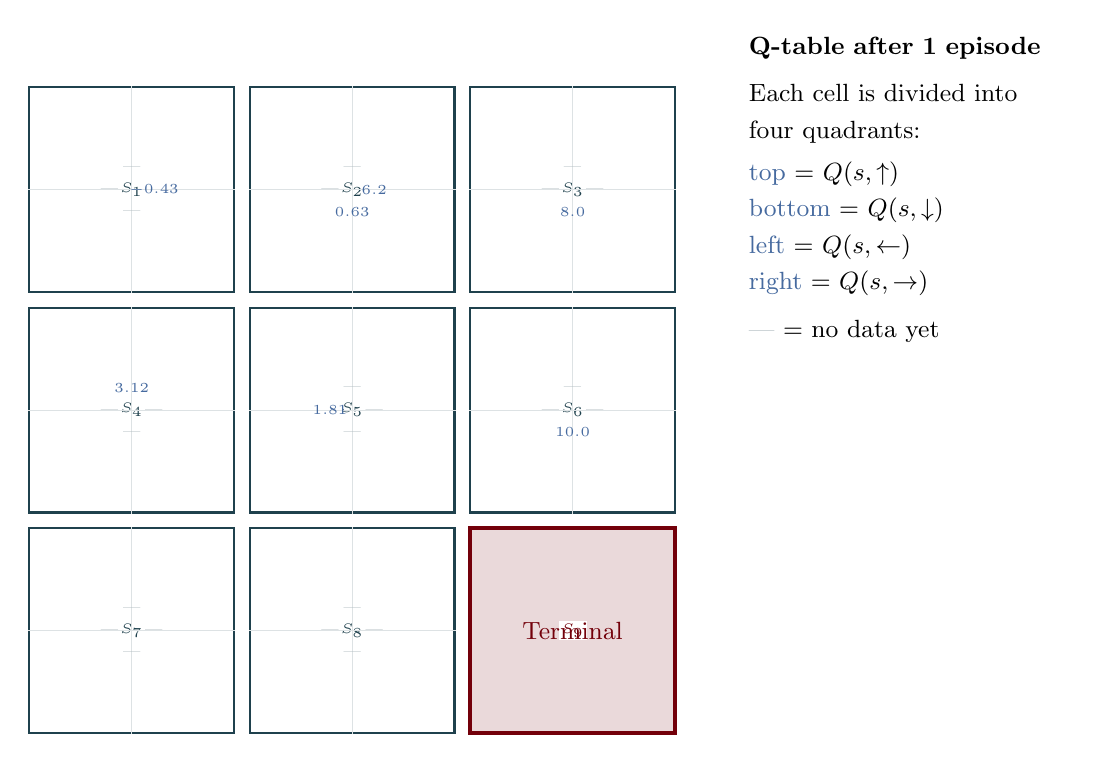
\begin{tikzpicture}[
    cell/.style={minimum size=2.6cm, draw=FlatDark, thick},
    goal/.style={cell, fill=Garnet!15, draw=Garnet, line width=1.5pt},
    empty/.style={cell, fill=LightGray},
    qval/.style={font=\tiny\bfseries, SecondaryBlue},
    qempty/.style={font=\tiny, FlatDark!35},
    slabel/.style={font=\tiny, FlatDark, fill=white, inner sep=1pt}
]
\def\cellspacing{2.8}
% Draw all 9 cells
\foreach \row/\rowidx in {2/0, 1/1, 0/2} {
    \foreach \col/\colidx in {0/0, 1/1, 2/2} {
        \pgfmathtruncatemacro{\idx}{\rowidx*3+\colidx+1}
        \ifnum\idx=9
            \node[goal] (s\idx) at (\col*\cellspacing, \row*\cellspacing) {};
        \else
            \node[cell] (s\idx) at (\col*\cellspacing, \row*\cellspacing) {};
        \fi
        % State label in center
        \ifnum\idx=9
            \node[slabel] at (s\idx.center) {\textcolor{Garnet}{$S_{\idx}$}};
        \else
            \node[slabel] at (s\idx.center) {$S_{\idx}$};
        \fi
        % Cross lines
        \ifnum\idx<9
            \draw[FlatDark!15] ([xshift=0pt]s\idx.west) -- ([xshift=0pt]s\idx.east);
            \draw[FlatDark!15] ([yshift=0pt]s\idx.south) -- ([yshift=0pt]s\idx.north);
        \fi
    }
}

% Q-values for S1: Right = -0.43
\node[qempty] at ([yshift=8pt]s1.center) {---};
\node[qempty] at ([yshift=-8pt]s1.center) {---};
\node[qempty] at ([xshift=-8pt]s1.center) {---};
\node[qval] at ([xshift=8pt]s1.center) {$-0.43$};

% Q-values for S2: Down = 0.63, Right = 6.2
\node[qempty] at ([yshift=8pt]s2.center) {---};
\node[qval] at ([yshift=-8pt]s2.center) {$0.63$};
\node[qempty] at ([xshift=-8pt]s2.center) {---};
\node[qval] at ([xshift=8pt]s2.center) {$6.2$};

% Q-values for S3: Down = 8.0
\node[qempty] at ([yshift=8pt]s3.center) {---};
\node[qval] at ([yshift=-8pt]s3.center) {$8.0$};
\node[qempty] at ([xshift=-8pt]s3.center) {---};
\node[qempty] at ([xshift=8pt]s3.center) {---};

% Q-values for S4: Up = 3.12
\node[qval] at ([yshift=8pt]s4.center) {$3.12$};
\node[qempty] at ([yshift=-8pt]s4.center) {---};
\node[qempty] at ([xshift=-8pt]s4.center) {---};
\node[qempty] at ([xshift=8pt]s4.center) {---};

% Q-values for S5: Left = 1.81
\node[qempty] at ([yshift=8pt]s5.center) {---};
\node[qempty] at ([yshift=-8pt]s5.center) {---};
\node[qval] at ([xshift=-8pt]s5.center) {$1.81$};
\node[qempty] at ([xshift=8pt]s5.center) {---};

% Q-values for S6: Down = 10.0
\node[qempty] at ([yshift=8pt]s6.center) {---};
\node[qval] at ([yshift=-8pt]s6.center) {$10.0$};
\node[qempty] at ([xshift=-8pt]s6.center) {---};
\node[qempty] at ([xshift=8pt]s6.center) {---};

% S7, S8: all empty
\node[qempty] at ([yshift=8pt]s7.center) {---};
\node[qempty] at ([yshift=-8pt]s7.center) {---};
\node[qempty] at ([xshift=-8pt]s7.center) {---};
\node[qempty] at ([xshift=8pt]s7.center) {---};

\node[qempty] at ([yshift=8pt]s8.center) {---};
\node[qempty] at ([yshift=-8pt]s8.center) {---};
\node[qempty] at ([xshift=-8pt]s8.center) {---};
\node[qempty] at ([xshift=8pt]s8.center) {---};

% S9: terminal
\node[font=\small, Garnet] at (s9.center) {Terminal};

% Legend
\node[anchor=west, font=\small, text width=4cm] at ([xshift=0.8cm]s3.east) {
    \textbf{Q-table after 1 episode}\\[4pt]
    Each cell is divided into\\
    four quadrants:\\[2pt]
    \textcolor{SecondaryBlue}{top} = $Q(s,\uparrow)$\\
    \textcolor{SecondaryBlue}{bottom} = $Q(s,\downarrow)$\\
    \textcolor{SecondaryBlue}{left} = $Q(s,\leftarrow)$\\
    \textcolor{SecondaryBlue}{right} = $Q(s,\rightarrow)$\\[4pt]
    \textcolor{FlatDark!35}{---} = no data yet
};
\end{tikzpicture}
\caption{Q-table visualization. Each cell shows estimated action values in four quadrants. Most (state, action) pairs remain unestimated (---) after a single episode.}
\label{fig:qtable_grid}
\end{figure}

% ============================================================
\section{The Exploration Problem}
% ============================================================

Look at Table~\ref{tab:qtable} and Figure~\ref{fig:qtable_grid} again. After one episode, we have estimates for only 8 out of 32 possible (state, action) pairs (8 non-terminal states $\times$ 4 actions = 32 pairs). The other 24 pairs have \textit{no data at all}. This is the \vocab{exploration problem}, and it is the central challenge of estimating action values with Monte Carlo methods.

\subsection{Why This Problem Didn't Exist for $V(s)$}

When estimating $V(s)$, every visit to state $s$ gives us useful data, regardless of which action the agent took. If the agent visits $S_2$ three times (taking Down, Right, and Left), all three visits contribute returns for estimating $V(S_2)$.

With $Q(s,a)$, things are different. Each visit to $S_2$ only provides data for the specific action taken. If the policy always chooses Right from $S_2$, we accumulate returns for $Q(S_2, \text{Right})$ but \textit{never} see $Q(S_2, \text{Up})$, $Q(S_2, \text{Down})$, or $Q(S_2, \text{Left})$. We cannot improve the policy because we do not know if those unexplored actions might actually be better.

\subsection{The Burger Place Analogy}

Imagine you always eat at the same burger restaurant. You know exactly how good the burgers are (you have a great estimate of $Q(\text{dinner}, \text{burgers})$), but you have no idea about the pizza place next door. Maybe the pizza is far better, maybe it is worse. You will never know unless you \textit{explore} by trying it. But if you always follow your current ``policy'' of choosing burgers, you are stuck with a potentially suboptimal choice forever.

This is exactly the exploration problem in MC estimation. A deterministic policy (one that always picks the same action in a given state) will never explore alternative actions, and thus can never discover if a different action is better.

\begin{tcolorbox}[memorybox={The Exploration Problem}]
When estimating $Q(s,a)$, a deterministic policy leaves many (state, action) pairs unvisited. Without data for these pairs, we cannot compare actions and cannot improve the policy. We need mechanisms to ensure that \textit{all} (state, action) pairs are visited sufficiently often. The two main solutions are \vocab{exploring starts} and \vocab{$\varepsilon$-greedy policies}.
\end{tcolorbox}

% ============================================================
\section{Solution 1: Exploring Starts}
% ============================================================

\begin{tcolorbox}[memorybox={Definition: Exploring Starts}]
\vocab{Exploring starts} requires that every (state, action) pair has a nonzero probability of being selected as the starting state and action of an episode. At the beginning of each episode, we randomly choose both a starting state $S_0$ and a starting action $A_0$, then follow the policy $\pi$ for all subsequent steps.
\end{tcolorbox}

The idea is simple: if we cannot guarantee that the policy will explore all (state, action) pairs during an episode, we can at least guarantee that every pair gets to be the \textit{first} step of some episode. Over many episodes, each pair will eventually be sampled as the starting pair, giving us at least one return for every $Q(s,a)$.

\subsection{How It Works}

At the start of each episode, uniformly sample a state $S_0$ from all non-terminal states and an action $A_0$ from all available actions. Take action $A_0$, observe the reward and next state, and then follow the current policy $\pi$ for all remaining steps until the episode terminates. Since we randomly select the starting pair, all 32 (state, action) pairs in our gridworld will eventually be sampled.

\subsection{Limitations}

Exploring starts is a useful theoretical tool, but it has a major practical limitation: it requires the ability to start an episode from \textit{any} state-action pair. In many real-world settings, this is impossible. You cannot restart a self-driving car in the middle of a highway facing the wrong direction. You cannot begin a chess game from an arbitrary board position. You cannot place a medical robot in the middle of a surgical procedure. Exploring starts assumes a level of control over the environment that we typically do not have.

\begin{tcolorbox}[examplebox={MC with Exploring Starts (MC ES) Pseudocode}]
\texttt{Initialize:} $Q(s,a) \leftarrow$ arbitrary, $\text{Returns}(s,a) \leftarrow$ empty list, for all $s, a$\\
\quad\quad\quad\; $\pi(s) \leftarrow$ arbitrary deterministic policy\\[4pt]
\texttt{For each episode:}\\
\quad Choose $S_0 \sim \text{Uniform}(\mathcal{S})$ and $A_0 \sim \text{Uniform}(\mathcal{A}(S_0))$ \hfill \textcolor{Garnet}{$\triangleleft$ exploring start}\\
\quad Generate episode from $S_0, A_0$ following $\pi$: $S_0, A_0, R_1, S_1, A_1, \ldots, S_T$\\
\quad $G \leftarrow 0$\\
\quad \texttt{For} $t = T-1, T-2, \ldots, 0$:\\
\quad\quad $G \leftarrow R_{t+1} + \gamma G$\\
\quad\quad \texttt{If} $(S_t, A_t)$ not in $\{(S_0,A_0), \ldots, (S_{t-1},A_{t-1})\}$:\\
\quad\quad\quad Append $G$ to $\text{Returns}(S_t, A_t)$\\
\quad\quad\quad $Q(S_t, A_t) \leftarrow \text{average}(\text{Returns}(S_t, A_t))$\\
\quad\quad\quad $\pi(S_t) \leftarrow \arg\max_a Q(S_t, a)$ \hfill \textcolor{Garnet}{$\triangleleft$ policy improvement}
\end{tcolorbox}

% ============================================================
\section{Solution 2: $\varepsilon$-Greedy Policies}
% ============================================================

\begin{tcolorbox}[memorybox={Definition: $\varepsilon$-Greedy Policy}]
An \vocab{$\varepsilon$-greedy policy} selects the greedy action (the one with the highest $Q$-value) with probability $1 - \varepsilon + \frac{\varepsilon}{|\mathcal{A}(s)|}$, and selects each of the other actions with probability $\frac{\varepsilon}{|\mathcal{A}(s)|}$. This ensures every action in every state has at least a $\frac{\varepsilon}{|\mathcal{A}(s)|}$ probability of being chosen.
\begin{align}
    \pi(a \mid s) = \begin{cases}
        1 - \varepsilon + \dfrac{\varepsilon}{|\mathcal{A}(s)|} & \text{if } a = \arg\max_{a'} Q(s, a') \\[8pt]
        \dfrac{\varepsilon}{|\mathcal{A}(s)|} & \text{otherwise}
    \end{cases}
\end{align}
\end{tcolorbox}

The $\varepsilon$-greedy policy is the most practical solution to the exploration problem. Instead of requiring special starting conditions, it builds exploration directly into the policy itself. At every step, there is a small chance of taking a random action, which means every (state, action) pair has a nonzero probability of being visited during normal operation.

\subsection{Worked Example}

Suppose $\varepsilon = 0.1$ and there are $|\mathcal{A}| = 4$ actions (Up, Down, Left, Right). The greedy action (say, Right) gets probability $1 - 0.1 + \frac{0.1}{4} = 0.925$. Each of the three non-greedy actions gets probability $\frac{0.1}{4} = 0.025$.

\begin{figure}[H]
\centering
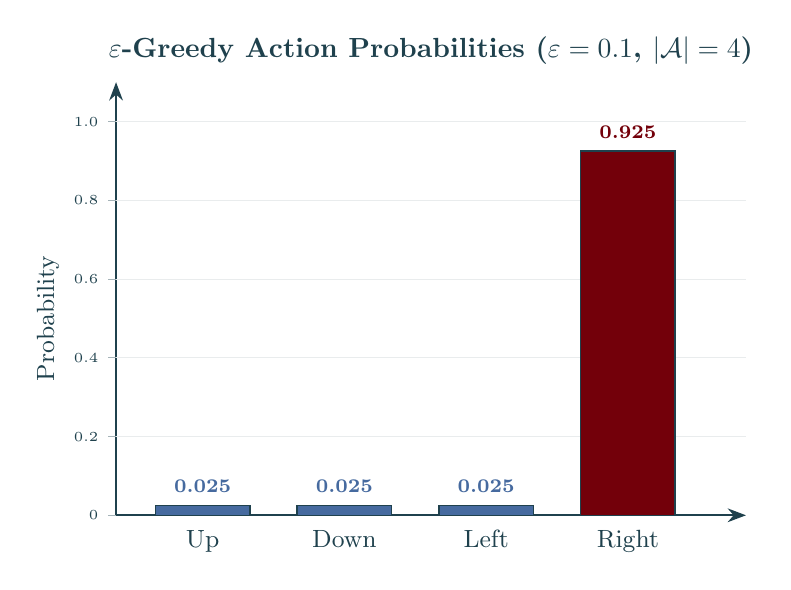
\begin{tikzpicture}[
    bar/.style={fill=SecondaryBlue, draw=FlatDark, line width=0.5pt},
    barg/.style={fill=Garnet, draw=FlatDark, line width=0.5pt},
    lbl/.style={font=\small, FlatDark},
    val/.style={font=\scriptsize\bfseries}
]
% Axes
\draw[-{Stealth}, FlatDark, line width=0.8pt] (-0.5, 0) -- (7.5, 0);
\draw[-{Stealth}, FlatDark, line width=0.8pt] (-0.5, 0) -- (-0.5, 5.5);
\node[font=\small, FlatDark, rotate=90, anchor=south] at (-1.1, 2.5) {Probability};

% Y-axis labels
\foreach \y/\lab in {0/0, 1/0.2, 2/0.4, 3/0.6, 4/0.8, 5/1.0} {
    \draw[FlatDark!40] (-0.6, \y) -- (-0.5, \y);
    \node[font=\tiny, FlatDark, anchor=east] at (-0.6, \y) {\lab};
}
% Gridlines
\foreach \y in {1,2,3,4,5} {
    \draw[FlatDark!10] (-0.5, \y) -- (7.5, \y);
}

% Bars: width=1.2, spacing=0.3
% Up: 0.025
\fill[bar] (0, 0) rectangle (1.2, 0.125);
\node[lbl, below=2pt] at (0.6, 0) {Up};
\node[val, above=1pt, SecondaryBlue] at (0.6, 0.125) {0.025};

% Down: 0.025
\fill[bar] (1.8, 0) rectangle (3.0, 0.125);
\node[lbl, below=2pt] at (2.4, 0) {Down};
\node[val, above=1pt, SecondaryBlue] at (2.4, 0.125) {0.025};

% Left: 0.025
\fill[bar] (3.6, 0) rectangle (4.8, 0.125);
\node[lbl, below=2pt] at (4.2, 0) {Left};
\node[val, above=1pt, SecondaryBlue] at (4.2, 0.125) {0.025};

% Right (greedy): 0.925
\fill[barg] (5.4, 0) rectangle (6.6, 4.625);
\node[lbl, below=2pt] at (6.0, 0) {Right};
\node[val, above=1pt, Garnet] at (6.0, 4.625) {0.925};
\node[font=\tiny, Garnet] at (6.0, 4.2) {(greedy)};

% Title
\node[font=\normalsize\bfseries, FlatDark, anchor=south] at (3.5, 5.6) {$\varepsilon$-Greedy Action Probabilities ($\varepsilon = 0.1$, $|\mathcal{A}| = 4$)};
\end{tikzpicture}
\caption{Probability distribution over actions for an $\varepsilon$-greedy policy with $\varepsilon = 0.1$. The greedy action gets 92.5\% of the probability mass, while each non-greedy action gets 2.5\%.}
\label{fig:epsilon_greedy}
\end{figure}

Even though the non-greedy probabilities are small (2.5\% each), they guarantee that over many episodes, every action in every state will be tried. This solves the exploration problem without requiring the ability to control the starting state.

\subsection{The Exploration--Exploitation Trade-Off}

The parameter $\varepsilon$ controls the balance between \vocab{exploration} (trying new actions to gather information) and \vocab{exploitation} (choosing the action we currently believe is best). A large $\varepsilon$ (e.g., 0.5) explores aggressively but makes many suboptimal choices. A small $\varepsilon$ (e.g., 0.01) mostly exploits the current best action but explores slowly. A common practice is to start with a larger $\varepsilon$ and gradually decay it over time, allowing the agent to explore broadly at first and then settle into a more refined policy.

\begin{tcolorbox}[examplebox={Choose $\varepsilon$-Greedy When...}]
\begin{itemize}[leftmargin=1.5em, itemsep=2pt]
    \item You \textit{cannot control the starting conditions} of episodes. This is the most common real-world scenario and is the primary motivation for $\varepsilon$-greedy over exploring starts.
    \item You want a \textit{simple, practical} exploration strategy that works in any environment.
    \item You are doing \textit{on-policy} learning, where the policy you are evaluating is the same policy generating the data. The $\varepsilon$-greedy policy generates its own exploratory data while still mostly exploiting what it has learned.
\end{itemize}
\end{tcolorbox}

% ============================================================
\section{Putting It All Together: MC Control Preview}
% ============================================================

We have now seen how to estimate action values $Q(s,a)$ from episodes and how to ensure all (state, action) pairs are explored. The natural next step is \vocab{Monte Carlo control}: using $Q$-value estimates to actually \textit{improve} the policy.

The MC control loop works as follows. First, generate an episode using the current policy (with exploration, via exploring starts or $\varepsilon$-greedy). Second, compute the returns and update the $Q$-table using first-visit or every-visit MC. Third, improve the policy by making it greedy (or $\varepsilon$-greedy) with respect to the updated $Q$-values: for each state $s$, set $\pi(s) = \arg\max_a Q(s,a)$.

This cycle of \textit{evaluation} (estimating $Q$) and \textit{improvement} (updating $\pi$) is called \vocab{generalized policy iteration (GPI)}. Each iteration brings the policy closer to optimal, and with sufficient episodes, the process converges to the optimal policy $\pi^*$ and optimal action-value function $Q^*$.

\begin{tcolorbox}[memorybox={Foundation for MC Control}]
Estimating $Q(s,a)$ is the essential building block of MC control methods. Without accurate $Q$-value estimates, we cannot compare actions and thus cannot improve the policy. The two exploration strategies (exploring starts and $\varepsilon$-greedy) ensure we get the data we need for every (state, action) pair. MC control methods, including on-policy and off-policy variants, will be covered in depth in a future guide.
\end{tcolorbox}

% ============================================================
\section{Key Takeaways}
% ============================================================

\begin{tcolorbox}[memorybox={Summary: From $V(s)$ to $Q(s,a)$}]
\textbf{$V(s)$ vs $Q(s,a)$:}
\begin{itemize}[leftmargin=1.5em, itemsep=2pt]
    \item $V(s)$ tells us how good a state is, but choosing actions from $V(s)$ requires a model of the environment.
    \item $Q(s,a)$ tells us how good each action is in each state, enabling \textit{model-free} action selection via $\arg\max_a Q(s,a)$.
    \item MC estimation of $Q(s,a)$ works the same as for $V(s)$, except we track returns for (state, action) pairs instead of just states.
\end{itemize}

\medskip

\textbf{Why exploration matters:}
\begin{itemize}[leftmargin=1.5em, itemsep=2pt]
    \item A deterministic policy only visits a fraction of (state, action) pairs, leaving most $Q$-values unestimated.
    \item Without estimates for all actions, we cannot compare them and thus cannot improve the policy.
\end{itemize}

\medskip

\textbf{Exploring starts vs $\varepsilon$-greedy:}
\begin{itemize}[leftmargin=1.5em, itemsep=2pt]
    \item \textit{Exploring starts} randomly selects the initial (state, action) pair for each episode. It guarantees coverage but requires the ability to control starting conditions, which is often impractical.
    \item \textit{$\varepsilon$-greedy policies} mix exploitation (choosing the best known action with probability $1 - \varepsilon + \varepsilon/|\mathcal{A}|$) with exploration (choosing a random action with probability $\varepsilon$). This is the practical default for ensuring exploration.
\end{itemize}
\end{tcolorbox}

\end{document}
